\documentclass[a4paper,UTF8]{article}
\usepackage{ctex}
\usepackage[margin=1.25in]{geometry}
\usepackage{color}
\usepackage{graphicx}
\usepackage{amssymb}
\usepackage{amsmath}
\usepackage{amsthm}
\usepackage{multirow}
\usepackage{url}
\usepackage[colorlinks,urlcolor=blue]{hyperref}
\usepackage{enumerate}
\usepackage{natbib}

%图片
\usepackage{subfigure}
\usepackage{float}
\usepackage{epstopdf}
\usepackage{caption}


\begin{document}
\title{《计算机图形学》系统报告}
\author{181860155 朱晓晴 \href{mailto:heloize@126.com}{heloize@126.com}}
\date{2020年12月}
\maketitle

\section{综述}
在9月提交中,主要完善了cg\underline{ }cli.py和cg\underline{ }algorithms.py两个模块。
在cg\underline{ }cli.py中,补充了对drawPolygon、drawEllipse等指令的解析。
在cg\underline{ }algorithms.py中,完成了线段绘制算法(draw\underline{ }line函数)
和椭圆绘制算法(draw\underline{ }ellipse函数)。

在10月提交中,主要完善了cg\underline{ }cli.py和cg\underline{ }algorithms.py两个模块。
在cg\underline{ }cli.py中,补充了对drawCurve、translate、rotate、scale和clip等指令的解析。
在cg\underline{ }algorithms.py中,完成了曲线绘制算法(draw\underline{ }curve函数)、
平移算法(translate函数)、旋转算法(rotate函数)、缩放算法(scale函数)和线段裁剪算法(clip函数)。
至此,所有指令的算法已全部完成。

在11月提交中,主要完成了cg\underline{ }gui.py中图形界面的基本功能,即将cg\underline{ }cli.py中的所有操作可视化。
同时,根据图形界面的显示需要,在cg\underline{ }algorithms.py中添加了相应的函数,
例如draw\underline{ }polygon\underline{ }gui。
至此,要求实现的功能已全部完成。

在12月提交中,对已有系统进行了优化,如修复bug、修改图形界面交互等。此外,对系统功能进行了拓展,添加了多边形填充、多边形裁剪等功能。


\section{算法介绍}
% 已完成或拟采用算法的原理介绍、自己的理解、对比分析等
\subsection{算法原理}
\subsubsection{绘制线段}
\textbf{要求:}根据给定两点$(x_0,y_0)$和$(x_1,y_1)$绘制线段。

绘制线段共需完成2种算法:DDA算法和Bresenham算法。

\textbf{DDA算法}

斜率$m=\frac{y_1-y_0}{x_1-x_0}$,
若$|m|\leqslant 1$,以$x_0<x_1$为例进行说明。
以单位间隔($x_{k+1}-x_k=1$)对$x$进行采样,并计算对应的$y$值:

$y_{k+1}=y_k+m\;(k=0,1,...)$

若$|m|>1$,以$y_0<y_1$为例进行说明。
以单位间隔($\Delta y=1$)对$y$进行采样,并计算对应的$x$值:

$x_{k+1}=x_k+\frac{1}{m}\;(k=0,1,...)$

\newpage
\textbf{Bresenham算法}

将$(x_0,y_0)$作为第一个点,
$m\geqslant 0$,决策参数初值为$p_0=2\Delta y-\Delta x$;
$m<0$,决策参数初值为$p_0=2\Delta y+\Delta x$。

$|m|\leqslant 1$时,以$x_0<x_1$的情况为例进行说明。

若$m\geqslant 0$,在每个$x_k$处进行检测$p_k$:

\hspace{2em}$p_k\geqslant 0$,下一个点为$(x_{k+1},y_{k}+1)$,
下一个决策参数$p_{k+1}=p_k+2\Delta y-2\Delta x$;

\hspace{2em}$p_k<0$,下一个点为$(x_{k+1},y_k)$,
下一个决策参数$p_{k+1}=p_k+2\Delta y$。

若$m<0$,在每个$x_k$处进行检测$p_k$:

\hspace{2em}$p_k\geqslant 0$,下一个点为$(x_{k+1},y_{k})$,
下一个决策参数$p_{k+1}=p_k+2\Delta y$;

\hspace{2em}$p_k<0$,下一个点为$(x_{k+1},y_{k}-1)$,
下一个决策参数$p_{k+1}=p_k+2\Delta y+2\Delta x$。


$|m|>1$时,以且$y_0<y_1$的情况为例进行说明。

若$m\geqslant 0$,在每个$y_k$处进行检测$p_k$:

\hspace{2em}$p_k\geqslant 0$,下一个点为$(x_{k}+1,y_{k+1})$,
下一个决策参数$p_{k+1}=p_k+2\Delta x-2\Delta y$;

\hspace{2em}$p_k<0$,下一个点为$(x_{k},y_{k+1})$,
下一个决策参数$p_{k+1}=p_k+2\Delta x$。

若$m<0$,在每个$y_k$处进行检测$p_k$:

\hspace{2em}$p_k\geqslant 0$,下一个点为$(x_{k},y_{k+1})$,
下一个决策参数$p_{k+1}=p_k+2\Delta x$;

\hspace{2em}$p_k<0$,下一个点为$(x_{k}-1,y_{k+1})$,
下一个决策参数$p_{k+1}=p_k+2\Delta x+2\Delta y$。


\subsubsection{绘制椭圆}
\textbf{要求:}根据给定的椭圆矩形包围框
左上角坐标$(x_0,y_0)$和右下角坐标$(x_1,y_1)$绘制椭圆。

\textbf{中点圆生成算法}

计算出椭圆中心$(x_c,y_c)$,长短轴径$r_x$和$r_y$。

(1)区域1中(|切线斜率|$\leqslant 1$)

计算得中心在原点的椭圆上的第一个点$(0,r_y)$。
在区域1每个$x_k$处,计算相应的决策参数:
\begin{equation*}
    p1_{k}=r_y^2(x_k+1)^2+r_x^2(y_k-\frac{1}{2})^2-r_x^2r_y^2
\end{equation*}
并对决策参数进行检测:

$p1_k<0$,下一个点为$(x_{k+1},y_k)$;

$p1_k\geqslant 0$,下一个点为$(x_{k+1},y_k-1)$。
\\循环直到$2r_y^2x\geqslant 2r_x^2xy$。

(2)区域2中(|切线斜率|$>1$)

在区域2每个$y_k$处,计算相应的决策参数:
\begin{equation*}
    p2_{k}=r_y^2(x_k+\frac{1}{2})^2+r_x^2(y_k-1)^2-r_x^2r_y^2
\end{equation*}
并对决策参数进行检测:

$p2_k\leqslant 0$,下一个点为$(x_k,y_{k+1})$;

$p2_k>0$,下一个点为$(x_k-1,y_{k+1})$。
\\循环直到$y=0$。

最后,计算出其他三个象限中的点,
并将所有的点平移到中心为$(x_c,y_c)$的椭圆轨迹上。


\subsubsection{绘制曲线}
\textbf{要求:}根据给定的若干控制点绘制曲线。

绘制曲线共需完成2种算法:Bezier算法和B-spline算法。

\textbf{Bezier曲线}

给定任一参数$u$,$u\in [0,1]$,利用de Castelijau递推算法来产生曲线上的点。
计算公式为:
\begin{equation*}
    P_i^r=
    \begin{cases}
        P_i & r=0\\
        (1-u)P_i^{r-1}+uP_{i+1}^{r-1} & r=1,2,...,n;\; i=0,1,...,n-r
    \end{cases}
\end{equation*}

$r=0$时,对应的顶点是曲线的控制点;
$r$不断增加时,每两个顶点生成一个新的顶点,
对应的顶点数递减,直到只剩下一个顶点。

在[0,1]内对$u$取值,对任一$u$的取值,
运行de Castelijau递推算法,得到Bezier曲线上的一个点。
最后,即可得到Bezier曲线。

\textbf{B-spline曲线}

实验要求B-Spline绘制出的曲线为三次均匀B样条曲线,设共给定$n+1$个控制点。

在定义域$[u_3,u_{n+1}]$中对$u$取值,对任一$u$的取值,
利用deBoox-Cox递推公式
\begin{equation*}
    B_{i,k}(u)
    =[\frac{u-u_i}{u_{i+k-1}-u_i}]B_{i,k-1}(u)
    +[\frac{u_{i+k}-u}{u_{i+k}-u_{i+1}}]B_{i+1,k-1}(u)
\end{equation*}
\begin{equation*}
    B_{i,1}(u)=
    \begin{cases}
    1 & u\in[u_i,u_{i+1}]\\
    0 & u\not\in[u_i,u_{i+1}]
    \end{cases}
\end{equation*}
计算出每个顶点的B-Spline基函数$B_{i,k}(u)$。
再根据B-Spline曲线公式
\begin{equation*}
    P(u)=\sum_{i=0}^nP_iB_{i,k}(u),u\in[u_3,u_{n+1}]
\end{equation*}
计算得曲线上的某一点。
最后,即可得到B-Spline曲线。


\subsubsection{图元平移}
\textbf{要求:}根据给定的平移向量$(dx,dy)$平移指定图元。

对于指定图元的任一图元参数$P_1(x_1,y_1)$,根据以下公式计算出新点$P_2(x_2,y_2)$的坐标:
\begin{equation*}
    \begin{cases}
        x_2=x_1+dx\\
        y_2=y_1+dy
    \end{cases}
\end{equation*}


\subsubsection{图元旋转}
\textbf{要求:}根据给定的旋转中心$(x,y)$和顺时针旋转角度$r$旋转指定图元。

首先,以$(x,y)$为原点旋转图元。
对于指定图元的任一图元参数$P_1(x_1,y_1)$,根据以下公式计算出点$P_2(x_2,y_2)$的坐标:
\begin{equation*}
    \begin{cases}
        x_2=(x1-x)cos(-r)-(y1-y)sin(-r)\\
        y_2=(x1-x)sin(-r)+(y1-y)cos(-r)
    \end{cases}
\end{equation*}

再以$(x,y)$为平移向量,平移$P_2(x_2,y_2)$得到新点$P_3(x_3,y_3)$:
\begin{equation*}
    \begin{cases}
        x_3=x_2+x\\
        y_3=y_2+y
    \end{cases}
\end{equation*}


\subsubsection{图元缩放}
\textbf{要求:}根据给定的缩放中心$(x,y)$和缩放倍数$s$缩放指定图元。

首先,以$(x,y)$为原点缩放图元。
对于指定图元的任一图元参数$P_1(x_1,y_1)$,根据以下公式计算出点$P_2(x_2,y_2)$的坐标:
\begin{equation*}
    \begin{cases}
        x_2=(x1-x)*s\\
        y_2=(x1-x)*s
    \end{cases}
\end{equation*}

再以$(x,y)$为平移向量,平移$P_2(x_2,y_2)$得到新点$P_3(x_3,y_3)$:
\begin{equation*}
    \begin{cases}
        x_3=x_2+x\\
        y_3=y_2+y
    \end{cases}
\end{equation*}


\subsubsection{线段裁剪}
\textbf{要求:}根据给定的裁剪窗口的
左上角顶点坐标$(x_{min},y_{max})$和右下角顶点坐标$(x_{max},y_{min})$
裁剪指定线段。

线段裁剪共需完成2种算法:Cohen-Sutherland算法和Liang-Barsky算法。

\textbf{Cohen-Sutherland算法}

Cohen-Sutherland算法的流程如图1所示,
对线段端点$(x_0,y_0)$和$(x_1,y_1)$编码的规则如图2所示。
\begin{figure}[H]
    \centering
    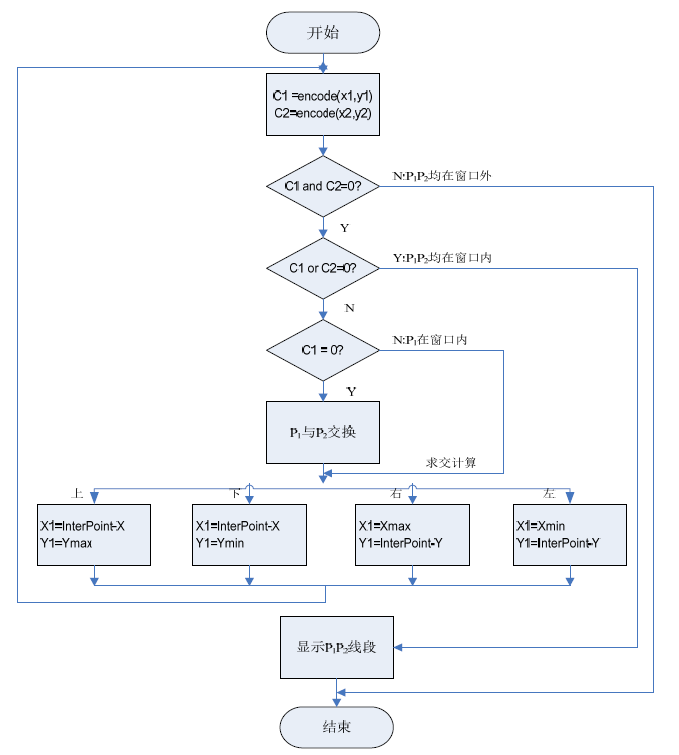
\includegraphics[scale=0.8]{cohen-sutherland-flow.PNG}
    \caption{Cohen-Sutherland算法流程图}
\end{figure}
\begin{figure}[H]
    \centering
    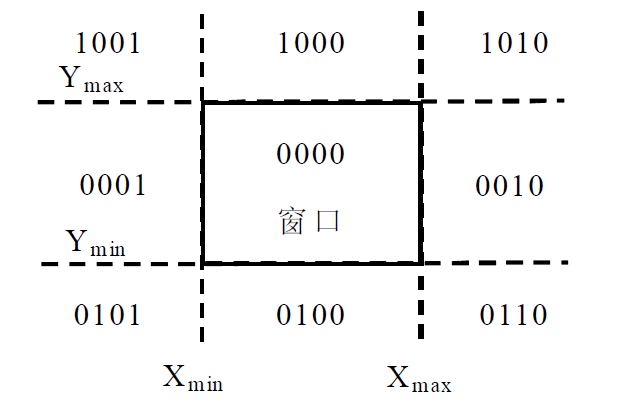
\includegraphics[scale=0.6]{cohen-sutherland-encode.PNG}
    \caption{区域编码}
\end{figure}


\textbf{Liang-Barsky算法}

定义如下8个参数:

\begin{equation*}
    \begin{cases}
        p_1=-\Delta x,q_1=x_0-x_{min}\\
        p_2=\Delta x,q_2=x_{max}-x_0\\
        p_3=-\Delta y,q_3=y_0-y_{min}\\
        p_4=\Delta y,q_4=y_{max}-y_0
    \end{cases}
\end{equation*}

初始化$u_1=0$,$u_2=1$。
对任一组$p_k$和$q_k$,做如下检测:

$p_k=0$时,若$q_k<0$,线段在裁剪窗口外,舍弃该线段,算法结束;

$p_k<0$时,令$u_1$为其本身和$\frac{q_k}{p_k}$中的较大值;

$p_k>0$时,令$u_2$为其本身和$\frac{q_k}{p_k}$中的较小值。

参数更新后,若$u_1>u_2$,舍弃该线段,算法结束。


\subsubsection{多边形填充}
\textbf{要求:}给定多边形顶点坐标列表,填充该多边形(返回需着色的内部像素点集合)。

多边形填充采用扫描转换填充算法,该算法的基本处理方式为:
对于每条穿过多边形的扫描线,计算出该扫描线与多边形各边的交点。
一般情况下,存在偶数个这样的交点(若共享顶点的两条边位于扫描线同侧,将该点记为两个交点)。
将这些交点从左至右配对,给每对交点区间内的像素点着色即可。

利用多边形各边的连贯特性,计算交点时可采用增量计算法来减少计算量。
如图3所示,两条相邻扫描线间$y$坐标的变化为:
\begin{equation*}
	y_{k+1}-y_k=1
\end{equation*}
扫描线交点的横坐标值$x_{k+1}$可从前一条扫描线交点的横坐标$x_{k}$计算得:
\begin{equation*}
	x_{k+1}=x_k+\frac{1}{m}
\end{equation*}
其中,$m$为$(x_k,y_k)$和$(x_{k+1},y_{k+1})$所在边的斜率。

\begin{figure}[H]
	\centering
	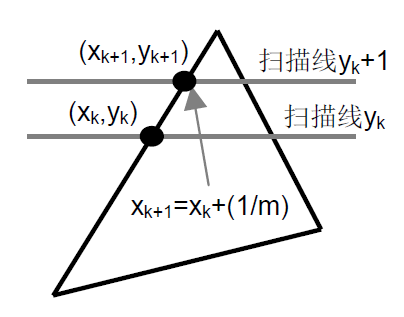
\includegraphics[scale=0.6]{polygon-fill.PNG}
	\caption{边的连贯性}
\end{figure}

多边形扫描转换填充算法的伪代码如下:

1.建立有序边表NET。
对于每个多边形顶点(按顺时针或逆时针顺序给出),如果该点的纵坐标小于前一个顶点的纵坐标,
则将三元组(该点横坐标,前一个点的纵坐标,两点确定的直线斜率的倒数),即$(x,ymax,k)$,加入该点纵坐标对应的扫描线在NET中的表项中。
对后一个顶点进行同样的操作。

2.对每一条扫描线(自下而上),用增量计算法更新活性边表AET表项的$x$值。

3.删除$ymax$等于当前扫描线$y$值的AET表项。

4.如果扫描线对应的NET表项非空,将其中的三元组合并到AET中,并按$x$值升序对AET中所有三元组排序。

5.给AET中排好序的三元组配对,将每对交点间的像素点加入需着色像素点的集合。
返回第2步,直到遍历完所有扫描线。


\subsubsection{多边形裁剪}
\textbf{要求:}给定多边形顶点坐标列表和裁剪窗口对角顶点坐标,返回裁剪后的多边形顶点坐标列表。

多边形裁剪采用了Sutherland-Hodgman算法,该算法对裁剪窗口的每一条边进行如下处理:

1.如图4(a)所示,以裁剪窗口的某一条边为界,将画布区域分为内侧和外侧。

2.如图4(b)所示,按序处理原多边形的每一条边,输出裁剪后的顶点坐标列表。
若后续要继续处理其他裁剪窗口便捷,将此步输出的顶点列表作为新的输入。

\begin{figure}[H]
	\centering
	\subfigure[输出顶点的确定方式]{
		\begin{minipage}{7cm}
			\centering
			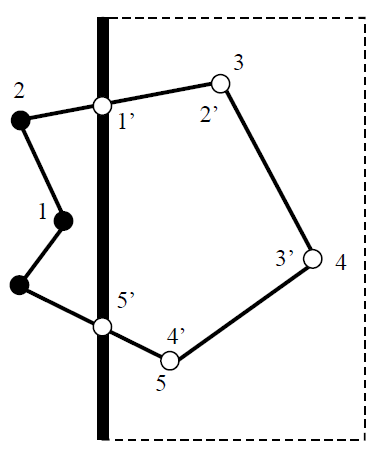
\includegraphics[scale=0.6]{polygon-clip-a.PNG}
	\end{minipage}}
	\subfigure[输出顶点的确定规则]{
		\begin{minipage}{7cm}
			\centering
			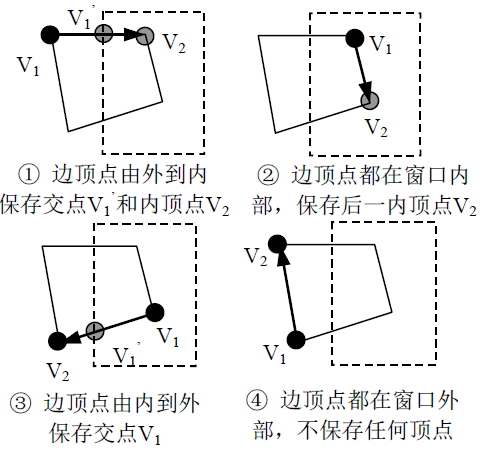
\includegraphics[scale=0.7]{polygon-clip-b.PNG}
	\end{minipage}}
	\caption{裁剪顶点的处理}
\end{figure}


        
\subsection{对比分析}
\subsubsection{绘制线段}
Naive算法以单位间隔对$x$取样,并根据直线方程计算出相应的$y$坐标,以此得到线段上所有的点。
这一过程需要做大量乘法运算,算法运行速度慢,且对硬件要求较高。
此外,Naive算法不对斜率绝对值大于1和小于1的两种情况区别处理,而是统一地以单位间隔对$x$取样。
因而,当斜率绝对值大于1时,易出现直线取样点稀疏的问题。

DDA算法针对上述缺陷做出了优化,它利用光栅特性消除了直线方程中的乘法,在$x$和$y$方向使用合适的增量逐步推导出各像素点的位置,两种算法的对比如图5所示。
然而,DDA算法仍有不足之处,算法中的浮点运算和取整操作十分耗时,且取整误差的积累会导致长线段的像素位置偏离实际位置。

Bresenham算法在每个已确定的像素点处计算决策参数,选择距离实际线段较近的点作为下一个绘制的点。
相较于DDA算法,这一做法有利于控制绘制出的直线对实际线段的偏离程度。

\begin{figure}[H]
    \centering
    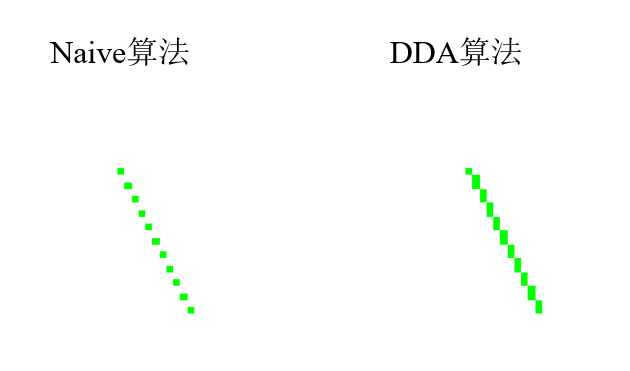
\includegraphics[scale=0.6]{naive-vs-dda.PNG}
    \caption{Naive算法和DDA算法效果对比}
\end{figure}

\subsubsection{绘制曲线}
绘制曲线使用了Bezier曲线和B-Spline曲线,两者在基函数和局部控制能力上存在较大差异。

在基函数方面,Bezier曲线基函数的次数始终等于控制顶点数减1,灵活性不足。
而B-Spline曲线基函数的次数则与控制顶点数无关。

在局部控制能力上,修改Bezier曲线的某一个控制顶点,会影响整条曲线的走向,Bezier曲线在局部性上有所欠缺。
而修改B-Spline曲线的某一个控制顶点,只影响曲线的某一部分,B-Spline曲线的局部性较好。

此外,在开发系统图形界面的过程中,相较于其他绘制和编辑图元的算法,曲线绘制算法的性能较差,尤其是B-Spline算法。在图形界面的刷新频率下,若单条曲线的控制点较多,或是曲线数目较多,系统易出现卡顿。

在开发过程中,考虑过优化曲线绘制算法性能。查阅相关资料后,得知通过分段绘制低阶Bezier曲线,可以显著减少浮点运算的次数。但是,鉴于正常情况下在本系统中绘制的曲线阶数应当不会超过20阶,优化后的算法性能并不会显著提升。此外,若为了进一步优化算法性能,仅令分段后的曲线具有一阶连续性,那么曲线的局部性将会加强,但平滑程度显著降低。因此,本系统仍然沿用2.1.3节中介绍的曲线绘制算法,不再另做优化。


\subsubsection{多边形裁剪}
本系统的多边形裁剪算法采用Sutherland-Hodgman算法,此算法能够正确处理对凸多边形的裁剪。
但对于凹多边形,则可能出现如图6所示的冗余线段。

出现这一情况的原因是Sutherland-Hodgman算法的输出为一个多边形,而不考虑裁剪后留下多个多边形的情况。
因此,图6(b)中的两个多边形之间存在冗余线段。
修正此算法的常见方法有对每条裁剪窗口边界进行拓扑检测,或是改用Weiler-Atherton双边裁剪算法,本系统暂未对Sutherland-Hodgman算法进行修正。

\begin{figure}[H]
	\centering
	\subfigure[裁剪前]{
		\begin{minipage}{7cm}
			\centering
			
\includegraphics[scale=0.8]{polygon-clip-c.PNG}
	\end{minipage}}
	\subfigure[裁剪后]{
		\begin{minipage}{7cm}
			\centering
			
\includegraphics[scale=0.8]{polygon-clip-d.PNG}
	\end{minipage}}
	\caption{Sutherland-Hodgman算法缺陷}
\end{figure}

系统未实现Weiler-Atherton双边裁剪算法,仅作简要介绍。
Weiler-Atherton算法按顺时针顺序建立多边形顶点表和裁剪窗口顶点表。
对多边形的每一条边,求其与裁剪窗口的交点,将交点标记为“入点”或“出点”,并将交点插入到多边形顶点表和裁剪窗口顶点表的相应位置。

然后,任取一个未追踪过的入点,沿多边形顶点表和裁剪窗口顶点表追踪出该点所在的多边形。
重复这一步骤,直到不存在未追踪过的入点。最终,得到裁剪后一个或多个多边形的顶点列表。


\section{系统介绍}
% 已完成或拟采用的系统框架、交互逻辑、设计思路等
\subsection{交互逻辑}
系统沿用demo的框架,即命令行和图形界面两种运行方式。

以命令行方式运行时,
系统逐行读取指令文件,解析指令
并调用cg\underline{ }algorithms.py模块中的相关算法。

以图形界面方式运行时,通过鼠标事件获取所需参数,
调用cg\underline{ }algorithms.py模块中的相关算法,
再以可视化方式呈现绘制或编辑结果。

下面简要介绍图形界面各个功能的实现逻辑,各功能的详细交互方式参见系统说明书。

\textbf{重置画布}

利用QDialog类生成输入窗口(见图7),得到输入的数据后,
首先清除画布中的所有图元,然后根据获得的数据重新设置画布的宽度和高度。
\begin{figure}[H]
    \centering
    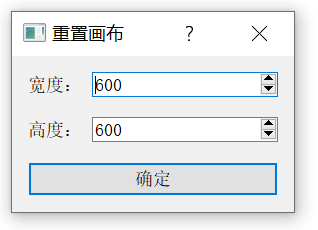
\includegraphics[scale=0.8]{reset-canvas.PNG}
    \caption{输入窗口}
\end{figure}

\newpage
\textbf{保存画布}

调用QFileDialog.getSaveFileName函数,显示出常见的文件保存界面(见图8)。
再调用QGraphicsView.grab函数截取画布,并将返回的数据保存为位图。
\begin{figure}[H]
    \centering
    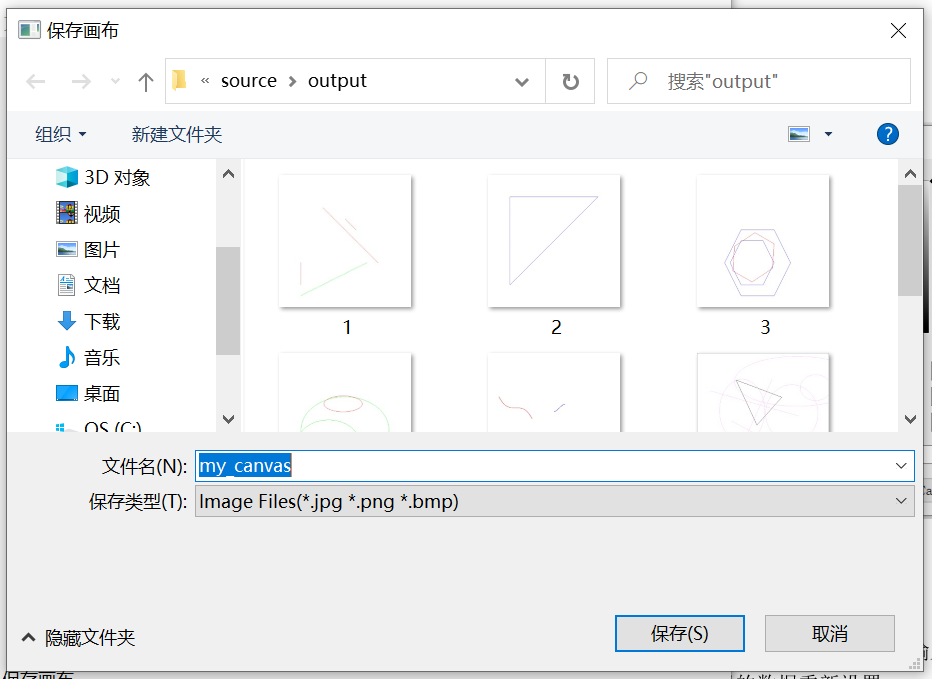
\includegraphics[scale=0.8]{save-canvas.PNG}
    \caption{文件保存窗口}
\end{figure}


\textbf{设置画笔}

调用QColorDialog.getColor函数,显示出常见的调板色界面(见图9),并记录下函数返回值,作为系统当前的画笔颜色。
为MyItem类添加成员变量color,以记录图元颜色。新建MyItem实例时,令该图元的颜色为系统当前的画笔颜色,即可实现要求的功能。

\begin{figure}[H]
	\centering
	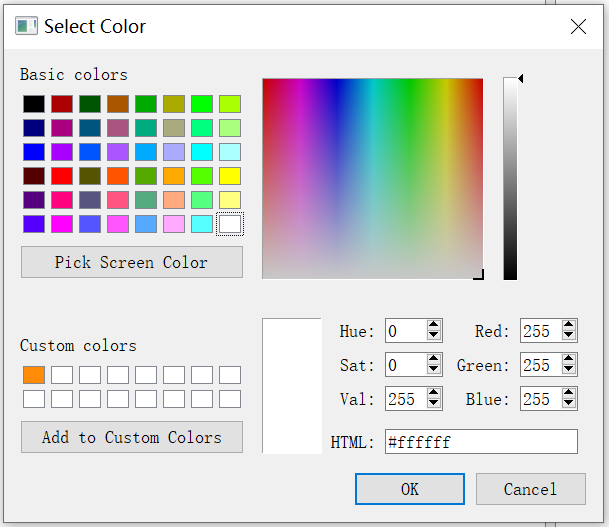
\includegraphics[scale=0.8]{select-color.PNG}
	\caption{颜色选择面板}
\end{figure}

\newpage
\textbf{绘制线段}

点击鼠标时,将当前坐标作为线段的两个端点。鼠标移动时,将线段第二个端点更新为当前坐标。将两个端点的坐标作为参数传给alg.draw\underline{ }line函数,得到线段。
\begin{figure}[H]
	\centering
	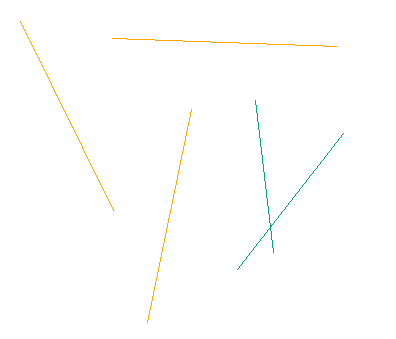
\includegraphics[scale=0.8]{draw-line.PNG}
	\caption{绘制线段示例}
\end{figure}


\textbf{绘制矩形}

点击鼠标时,将当前坐标作为矩形的两个对角顶点。鼠标移动时,将第二个对角顶点更新为当前坐标。确定对角顶点后,计算出矩形的四个顶点,作为参数传给alg.draw\underline{ }polygon函数,得到矩形。
\begin{figure}[H]
	\centering
	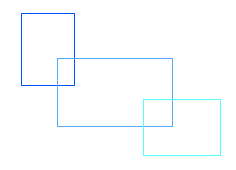
\includegraphics[scale=0.8]{draw-rectangle.PNG}
	\caption{绘制矩形示例}
\end{figure}


\textbf{绘制多边形}

点击鼠标时,如果当前的点在第一个顶点为圆心半径为10的圆内,且当前已确定的顶点数不小于3,则认为已经绘制完毕;否则,把当前坐标加入多边形的顶点列表。
鼠标移动时,将顶点列表的最后一个坐标更新为当前坐标。
\begin{figure}[H]
    \centering
    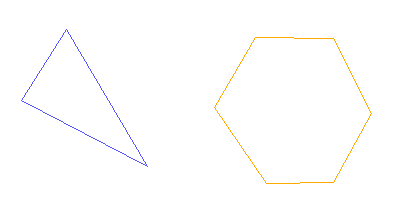
\includegraphics[scale=0.8]{draw-polygen.PNG}
    \caption{绘制多边形示例}
\end{figure}
\newpage
\textbf{绘制椭圆}

点击鼠标时,将当前坐标作为椭圆绑定矩形的对角顶点坐标。鼠标移动时,将第二个对角顶点坐标更新为当前坐标。将两个顶点的坐标作为参数传给alg.draw\underline{ }ellipse函数,得到椭圆。
\begin{figure}[H]
    \centering
    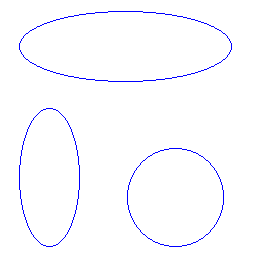
\includegraphics[scale=0.8]{draw-ellipse.PNG}
    \caption{绘制椭圆示例}
\end{figure}


\textbf{绘制曲线}

点击鼠标时,把当前坐标加入曲线的控制点列表。鼠标移动时,将控制点列表的最后一个坐标更新为当前坐标。鼠标点击其他绘制或编辑功能时,绘制结束。绘制曲线或曲线被选中时,会显示曲线控制点。
\begin{figure}[H]
    \centering
    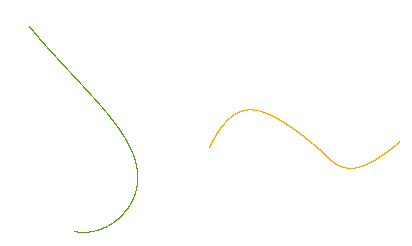
\includegraphics[scale=0.8]{draw-curve.PNG}
    \caption{绘制曲线示例}
\end{figure}


\textbf{平移}

点击鼠标时,若当前左边在选中图元的绑定矩形内,将当前坐标作为平移向量的起点和终点坐标。鼠标移动时,将平移向量的终点坐标更新为当前坐标。将平移向量的坐标作为参数传给alg.translate函数,得到平移后的图元。
\begin{figure}[H]
    \centering
    \subfigure[平移前]{
    \begin{minipage}{7cm}
        \centering
        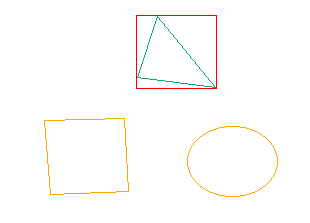
\includegraphics[scale=0.8]{before-translate.PNG}
    \end{minipage}}
    \subfigure[平移后]{
        \begin{minipage}{7cm}
            \centering
            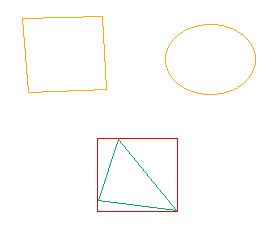
\includegraphics[scale=0.8]{after-translate.PNG}
        \end{minipage}}
        \caption{平移示例}
\end{figure}


\textbf{旋转}

将图元绑定矩形的中心作为旋转中心,点击鼠标时将当前坐标作为旋转弧线的起点和终点,移动鼠标时将弧线的终点更新为当前坐标。
将旋转中心坐标和根据弧线计算出的旋转角度作为参数传给alg.rotate函数,得到旋转后的图元。
\begin{figure}[H]
    \centering
    \subfigure[旋转前]{
    \begin{minipage}{7cm}
        \centering
        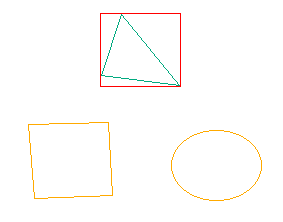
\includegraphics[scale=0.8]{before-rotate.PNG}
    \end{minipage}}
    \subfigure[旋转后]{
        \begin{minipage}{7cm}
            \centering
            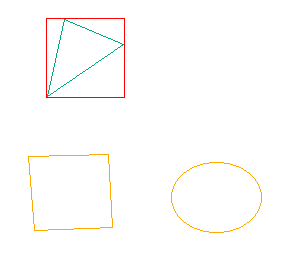
\includegraphics[scale=0.8]{after-rotate.PNG}
        \end{minipage}}
        \caption{旋转示例}
\end{figure}


\textbf{缩放}

将图元绑定矩形的中心作为缩放中心,点击鼠标时将当前坐标作为缩放线段的起点和终点,移动鼠标时将缩放线段的终点更新为当前坐标。
令缩放倍数等于缩放线段长度与80的比值,将缩放中心坐标和缩放倍数作为参数传给alg.scale函数,得到缩放后的图元。
\begin{figure}[H]
    \centering
    \subfigure[缩放前]{
    \begin{minipage}{7cm}
        \centering
        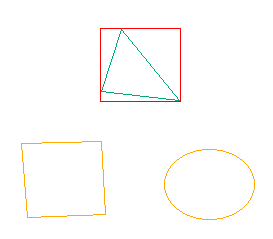
\includegraphics[scale=0.8]{before-scale.PNG}
    \end{minipage}}
    \subfigure[缩放后]{
        \begin{minipage}{7cm}
            \centering
            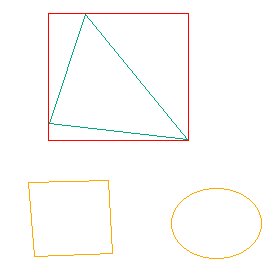
\includegraphics[scale=0.8]{after-scale.PNG}
        \end{minipage}}
        \caption{缩放示例}
\end{figure}


\textbf{裁剪}

点击鼠标时,将当前坐标作为裁剪窗口的对角顶点坐标。鼠标移动时,将裁剪窗口的第二个对角顶点坐标更新为当前坐标。
将两个顶点坐标作为参数传给alg.clip函数,得到裁剪后的线段。
\begin{figure}[H]
    \centering
    \subfigure[裁剪前]{
    \begin{minipage}{7cm}
        \centering
        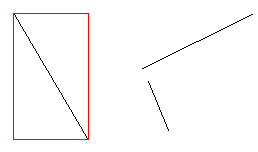
\includegraphics[scale=0.8]{before-clip.PNG}
    \end{minipage}}
    \subfigure[裁剪后]{
        \begin{minipage}{7cm}
            \centering
            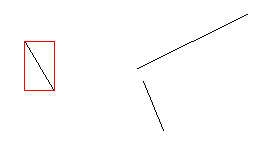
\includegraphics[scale=0.8]{after-clip.PNG}
        \end{minipage}}
        \caption{线段裁剪示例}
\end{figure}


\textbf{多边形填充}

将选中多边形的fill标记置为True。
多边形的paint函数被调用时,如果fill标记为True,
会调用alg.polygon\underline{ }fill函数,得到需要着色的内部像素点列表,并将其着色。

\begin{figure}[H]
	\centering
	\subfigure[填充前]{
		\begin{minipage}{7cm}
			\centering
			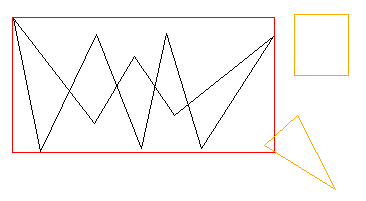
\includegraphics[scale=0.65]{before-polygon-fill.PNG}
	\end{minipage}}
	\subfigure[填充后]{
		\begin{minipage}{7cm}
			\centering
			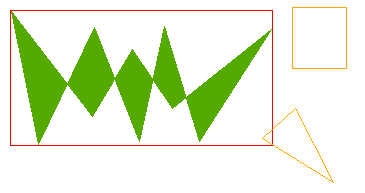
\includegraphics[scale=0.65]{after-polygon-fill.PNG}
	\end{minipage}}
	\caption{多边形填充示例}
\end{figure}


\textbf{多边形裁剪}

点击鼠标时,将当前坐标作为裁剪窗口的对角顶点坐标。鼠标移动时,将裁剪窗口的第二个对角顶点坐标更新为当前坐标。
将两个顶点坐标作为参数传给alg.polygon\underline{ }clip函数,得到裁剪后的多边形。
\begin{figure}[H]
	\centering
	\subfigure[裁剪前]{
		\begin{minipage}{7cm}
			\centering
			
\includegraphics[scale=0.65]{before-polygon-clip.PNG}
	\end{minipage}}
	\subfigure[裁剪后]{
		\begin{minipage}{7cm}
			\centering
			
\includegraphics[scale=0.65]{after-polygon-clip.PNG}
	\end{minipage}}
	\caption{多边形裁剪示例}
\end{figure}


\textbf{删除}

将选中图元从scene中删除即可。\\


\textbf{复制}

将选中图元添加到画布剪切板,待后续粘贴。\\

\textbf{粘贴}

根据剪切板中的图元的信息(图元类型、顶点列表、颜色等),新建新的图元。
新图元的位置较原图元的位置有一定偏差,用于区分两个图元。
\begin{figure}[H]
	\centering
	\subfigure[粘贴前]{
		\begin{minipage}{7cm}
			\centering
			
\includegraphics[scale=0.65]{before-paste.PNG}
	\end{minipage}}
	\subfigure[粘贴后]{
		\begin{minipage}{7cm}
			\centering
			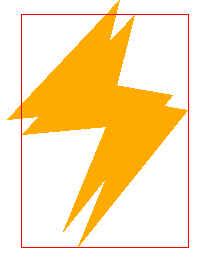
\includegraphics[scale=0.65]{after-paste.PNG}
	\end{minipage}}
	\caption{粘贴示例}
\end{figure}



\subsection{设计思路}
系统设计有两大主要方向:使系统功能更强大、使系统使用更便捷。

在拓展系统功能方面,本系统在实现基本功能的基础上,添加了绘制矩形、多边形填充、多边形裁剪、复制和粘贴等附加功能。

在优化用户体验方面,本系统在图形界面中进行了若干优化,如实现鼠标点选图元、显示曲线控制点等,优化细节参见4.3节。


\section{补充内容}
\subsection{附加功能}
系统在图元绘制、图元编辑和交互方式三个方面实现了以下附加功能:

\hspace*{2em}图元绘制:绘制矩形

\hspace*{2em}图元编辑:多边形填充、多边形裁剪、删除图元、复制、粘贴

\hspace*{2em}交互方式:鼠标点选

其中,图元绘制和图元编辑中添加的功能已在3.2节中详细介绍交互逻辑,具体的交互操作参见系统说明书。
此处将对鼠标点选功能进行简要介绍:当系统空闲时,即不在进行系统设置、图元绘制和图元编辑操作时,点击画布任意处,如果该处有图元,该图元被选中并显示绑定矩形。

\subsection{界面设计}
本系统保留了demo中的菜单栏,并添加了工具栏(见图22)。
工具栏提供了本系统所有功能的接口,以图标呈现,易于理解且便于用户操作。
\begin{figure}[H]
	\centering
	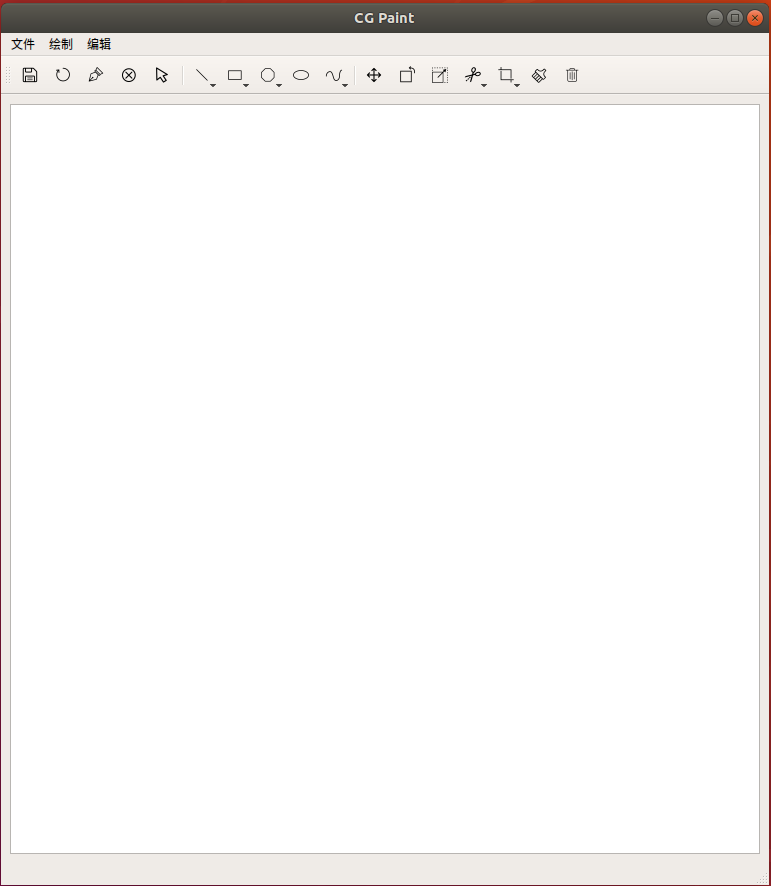
\includegraphics[scale=0.5]{gui.PNG}
	\caption{图形界面}
\end{figure}

\subsection{交互设计}
本节将介绍系统图形界面若干易用或有特色的交互。

鼠标点选:本系统取消了demo中的图元列表,支持鼠标点选图元。

连续绘制、编辑:参考现有的商用画图系统,本系统支持用户连续绘制、编辑图元(除线段裁剪、多边形裁剪外)。

工具栏:demo中以菜单栏实现对系统功能的选择,但操作不够简便。
因此,本系统添加了工具栏,以图标形式展示系统功能。
其中,系统设置和图元绘制功能基本沿用常见画图系统的图标,方便用户识别、选择。
需要特别提及的是鼠标点击图标,即工具栏左起第五个图标。
本系统支持用户连续绘制、编辑图元,点击这一图标用户即可使系统进入空闲状态,若多边形、曲线等图元未绘制完成,系统将自动处理。系统进入空闲状态后,用户可通过鼠标点击选择图元。

矩形绘制:通过多边形绘制也可绘制出矩形,但水平、垂直线段不易通过鼠标绘制出,因此系统添加了绘制矩形的功能。矩形绘制没有沿用多边形绘制时逐个点击顶点的交互方式,而是直接拖拽出矩形对角线即可。然而,矩形未绘制结束时,系统并不以多边形的形式保存它,因为矩形形状和位置的频繁变动与多边形绘制算法不适配,会导致画布显示的矩形有偏差。因此,系统先将该图元以矩形类型暂存,只保存对角顶点坐标,待绘制完毕再修改为多边形类型。

多边形绘制:多边形绘制时,仅当用户再次点击多边形第一个顶点(允许一定误差)时,系统才认为多边形绘制结束。尽管此交互需要用户额外点击一次,且存在点击误差较大导致绘制未按预期结束的情况,但此交互便于用户观察多边形绘制进度,以及各顶点间的位置关系。

曲线绘制:曲线绘制或曲线被选中时,系统会显示曲线的控制点,便于用户观察控制点位置,以及控制点对曲线的影响。

平移:鼠标拖出的平移向量的起点在图元绑定矩形内,平移操作才会成功。

旋转、缩放:起初,在图形界面旋转或缩放图元时,用户需要先指定一个旋转或缩放中心,在拖拽鼠标进行旋转或缩放。尽管上述交互符合实验要求,但操作不简易,且与常见画图系统差异较大,不易于用户操作。因此,最后选择以图元绑定矩形的中心为旋转、缩放中心。



\section{总结}
在系统开发过程中,运用了目前已讲到图形学基础知识,并自学了解了若干绘制图元和编辑图元的算法,以及图形界面开发的知识。
通过实现所有指令的算法和图形界面,加深了对图形显示原理的理解。
同时,通过反复测试找出了之前提交代码中的若干错误,如公式错误、功能异常等。
在纠正代码错误的过程中,加深了对算法公式推导过程和Python语言的理解程度。

此外,为了使得系统界面更加美观、交互更加易用,开发过程中也做出了较多测试和修改,使得系统更接近现有的常见商用画图系统。这一过程并不因图形界面的简易而变得轻松,加深了我对图形界面开发的了解。
\\\\\\



\bibliographystyle{plain}
\begin{thebibliography}{99}
% 注明在实现作业过程中使用的参考资料,包括技术博客等
\bibitem{ref1} 孙正兴等. 计算机图形学教程[M]. 机械工业出版社, 2006.
\bibitem{ref2} Qt 5.15手册\\\url{https://doc.qt.io/qt-5/index.html}
\bibitem{ref3} 计算向量夹角\\\url{https://blog.csdn.net/qq_42423940/article/details/83757427}
\bibitem{ref4} QListWidget右键菜单\\\url{https://blog.csdn.net/qq_42365249/article/details/106651354}
\bibitem{ref5} PyQt 5菜单栏、工具栏和状态栏使用\\\url{https://www.cnblogs.com/ygzhaof/p/10070523.html}
\bibitem{ref6} QToolButtton简介\\\url{https://blog.csdn.net/qq_17351161/article/details/102917153}
\bibitem{ref7} 多边形填充算法\\\url{https://blog.csdn.net/keneyr/article/details/83747501}
\bibitem{ref8} 多边形裁剪Weiler-Atherton算法\\\url{https://blog.csdn.net/yangxi_pekin/article/details/37738219} 
\end{thebibliography}

\end{document}